
\subsection{Problématique}

\begin{frame}{Problématique scientifique}
    \begin{columns}
        \begin{column}{0.56\linewidth}
            \begin{description}
                \setlength\itemsep{1em}
                \item[Difficultés]
                    \begin{itemize}
                        \item Petits robots humanoïdes
                        \item Nombreuses imperfections
                    \end{itemize}
                \item[Problème] 
                    \begin{itemize}
                        \item Réduire écart comportement estimé/désiré et réalité
                        \item Méthodes d'apprentissage
                    \end{itemize}
                \item[Applications] Compétition RoboCup
                    \begin{itemize}
                        \item Déplacement du robot (odométrie)
                        \item Modèle de caméra
                        \item Synthèse de mouvements dynamiques
                    \end{itemize}
                \item[Contexte]
                    \begin{itemize}
                        \item Puissance de calcul limité (autonomie)
                        \item Solutions opérationnelles
                    \end{itemize}
            \end{description}
        \end{column}
        \begin{column}{0.44\linewidth}
            \centering
            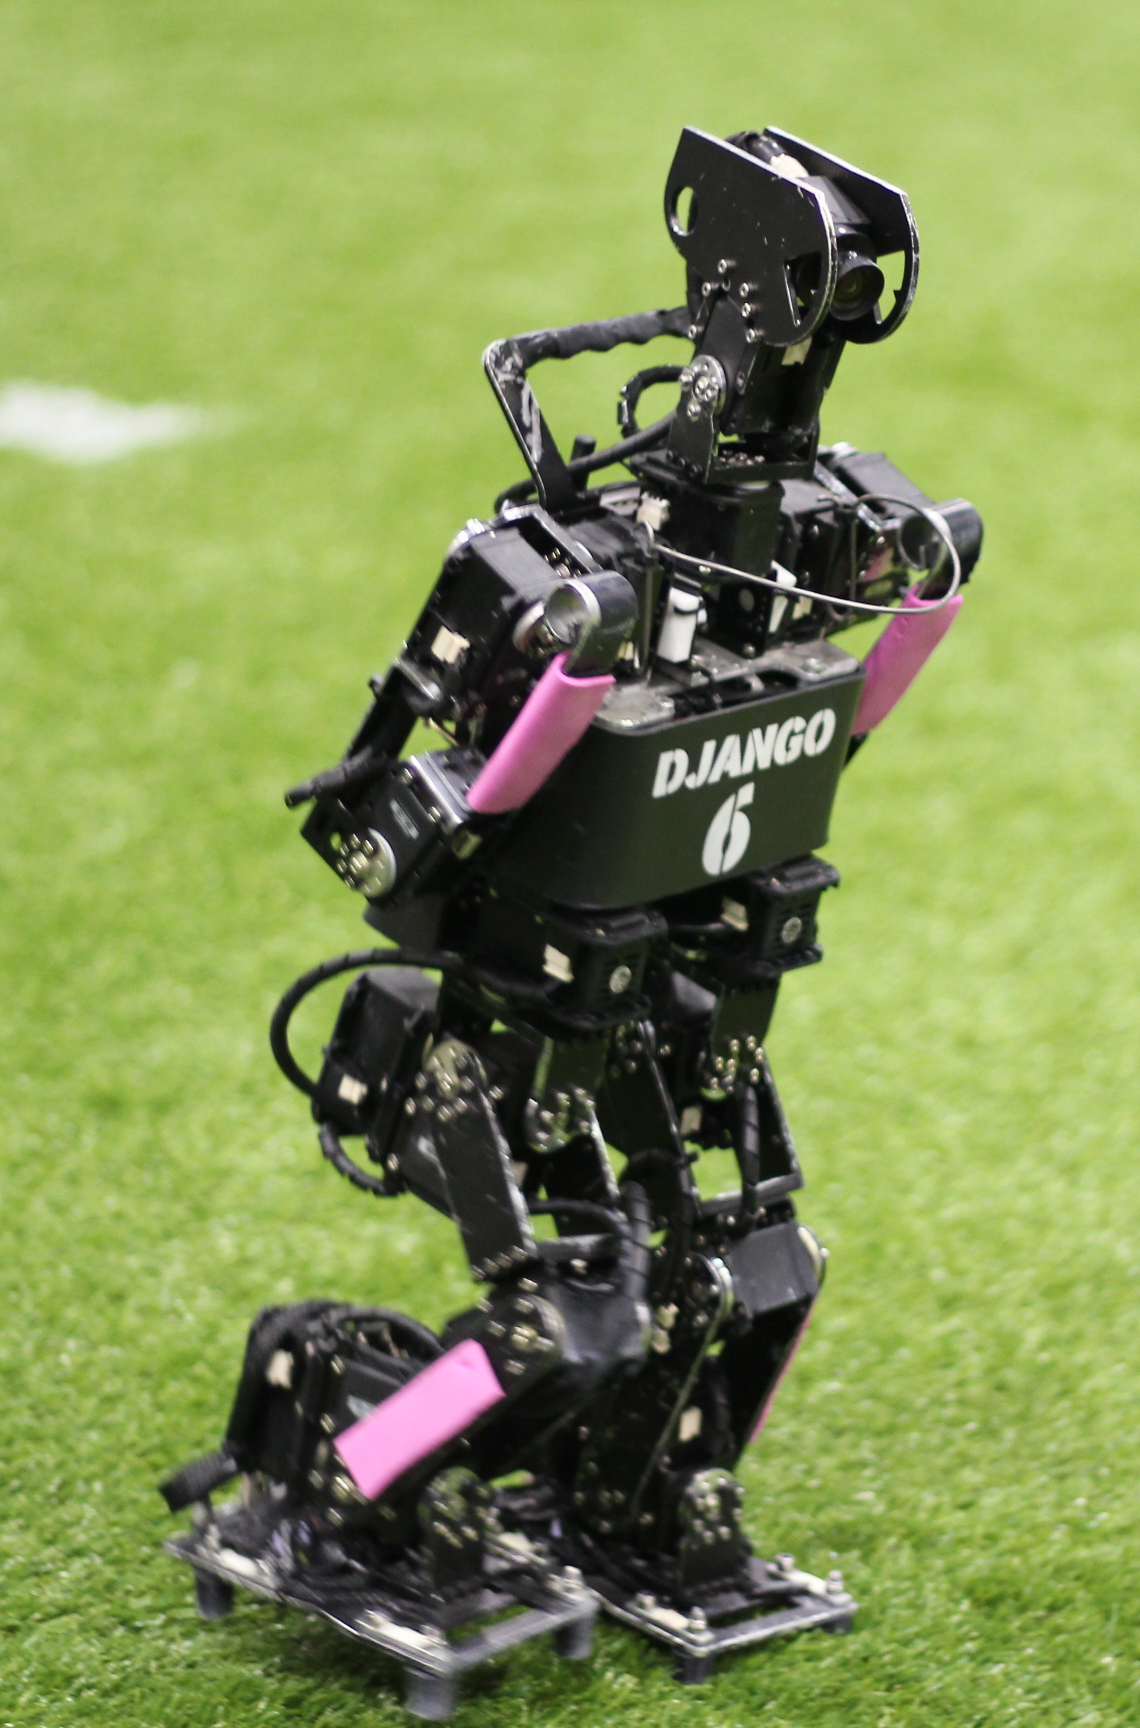
\includegraphics[height=4.0cm]{../media/sigmaban_1_6.png}
            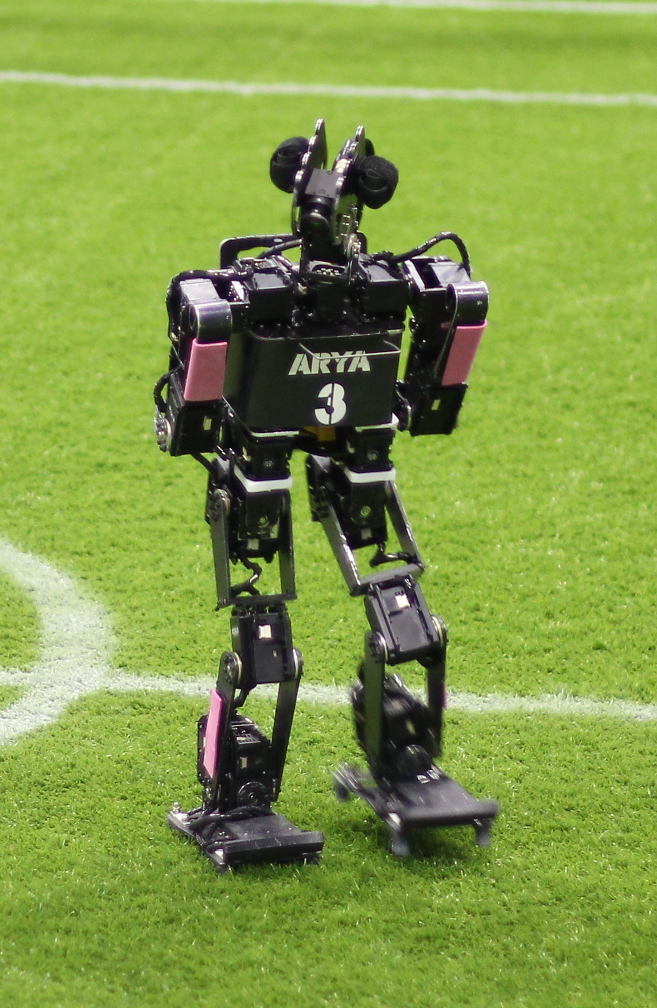
\includegraphics[height=4.0cm]{../media/grosban_1_2.png}
        \end{column}
    \end{columns}
\end{frame}

